\documentclass{standalone}
\usepackage{tikz}

\begin{document}
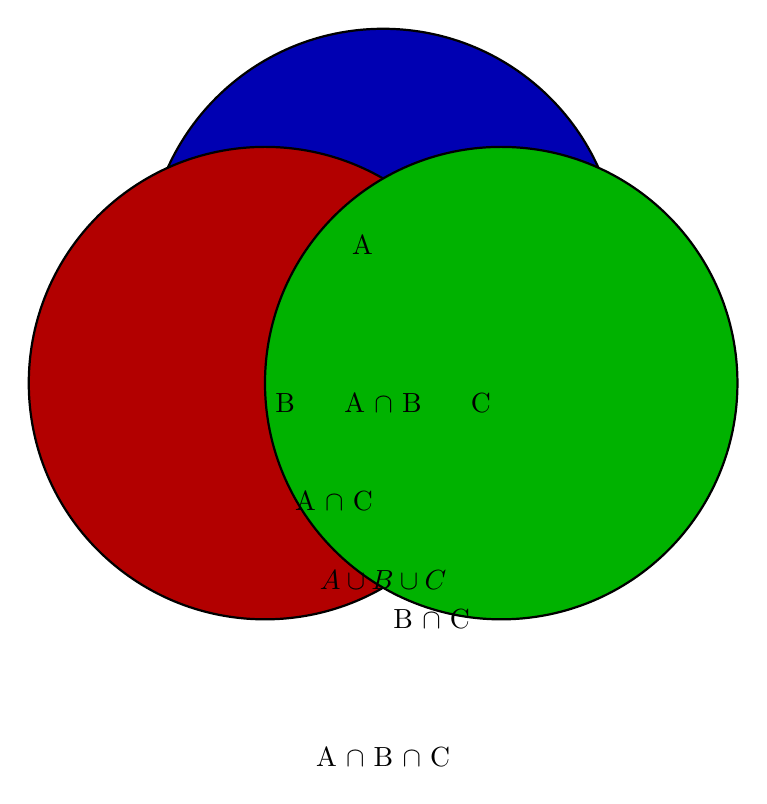
\begin{tikzpicture}[thick, scale=1.5]

% Define the colors for each set
\colorlet{SetA}{blue!70!black}
\colorlet{SetB}{red!70!black}
\colorlet{SetC}{green!70!black}

% Draw the circles
\draw[fill=SetA] (0,0) circle[radius=2cm];
\draw[fill=SetB] (-1,-1) circle[radius=2cm];
\draw[fill=SetC] (1,-1) circle[radius=2cm];

% Add labels for each set
\node at (0,0) [above left] {A};
\node at (-1,-1) [below right] {B};
\node at (1,-1) [below left] {C};

% Add labels for the intersection regions
\node at (0,-1) [below] {A $\cap$ B};
\node at (0,-2) [left] {A $\cap$ C};
\node at (0,-3) [right] {B $\cap$ C};
\node at (0,-4) [below] {A $\cap$ B $\cap$ C};

% Add the outermost region
\node at (0,-2.5) [below] {$A \cup B \cup C$};

\end{tikzpicture}
\end{document}